\documentclass[a4paper]{article} %format de la feuille + type de document https://en.wikibooks.org/wiki/LaTeX/Document_Structure#Document_classes
%packages nécessaire pour nos besoins
\usepackage[utf8]{inputenc}
\usepackage[T1]{fontenc}
\usepackage[english,french]{babel}
\usepackage{amsmath}
\usepackage{amssymb,amsfonts,textcomp}
\usepackage{color}
\usepackage{array}
\usepackage{supertabular}
\usepackage{hhline}
\usepackage{hyperref}
\usepackage{capt-of}
\usepackage[pdftex]{graphicx}
\usepackage{sectsty}
\usepackage{tcolorbox}
\usepackage{textcomp}
\usepackage{courier}
\usepackage[font={small,it}]{caption}
\usepackage{float}
\usepackage{graphicx}
\usepackage{caption}



%Définition des couleurs
\definecolor{havelockBlue}{rgb}{0.004, 0.42, 0.73}
\definecolor{Monokaimagenta}{rgb}{0.86,0.08,0.24}

%utilisation de la couleur définie avant
%toutes les sections auront cette couleur
\sectionfont{\color{havelockBlue}}
\subsectionfont{\color{havelockBlue}}
%début du document
\begin{document}

%début d'un titre
\begin{titlepage}
            %centre les éléments
	\centering
	
	{\scshape\LARGE \color{Monokaimagenta} Laboratoire \\ Universal Asynchronous Receiver Transmitter \par}
	
	%espace vertical de 1 mms
	\vspace{1cm}
	
	{\Large\itshape Johanna Melly \& Sven Rouvinez\par}
	
	%http://www.personal.ceu.hu/tex/spacebox.htm
	\vfill
	Professeur\par
	%met le texte en gras 
	\textbf{Carlos Andrés Pena} \par% ajoute une ligne 
	\vspace{1cm}
	Assistant\par
	\textbf{Gaëtan Matthey}
	
	\vfill

            %affiche la date actuelle
	{\large \today\par}
	
%fin de la page de titre
\end{titlepage}

%démarre un chapitre, les nombres se mettent automatiquement et seront incrémenté quand un autre \section est rencontré
%voir https://en.wikibooks.org/wiki/LaTeX/Document_Structure#Sectioning_commands
\section{Description générale}
On appelle « trame » une suite de bits envoyés en série. Cette trame comprend dans l’ordre :
\begin{itemize}
\item Le « start-bit » toujours égal à 0.
\item Les bits de donnée (sur n bits) à transmettre.
\item Le bit de parité facultatif (non demandé dans ce labo).
\item Le bit de stop égal à 1.
\end{itemize}
De plus, l’état de repos de la ligne est fixé à 1.
\\ 
\begin{figure}[H]
    \centering
    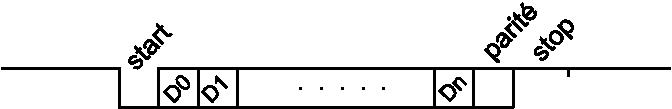
\includegraphics[width=.8\textwidth]{src/uart_1.jpg}
    \captionof{figure}{trame}
    \label{fig:trame}
\end{figure}


%saut à la ligne


%début d'un encadré avec la couleur définie plus haut
\begin{tcolorbox}[colframe=Monokaimagenta,colback=white]
Nous réalisons la partie récepteur. Le circuit se compose d'un shift register, de deux compteurs, un registre de sortie et un machine à états pour le contrôle.\\
Le début de la communication démarre lorsque que le contrôle reçoit un $0$.

\begin{itemize}
    \item    Après un reset, le registre de sortie contient la valeur $0$
    \item    Détection du front descendant sur l'entrée série provoqué par le \textbf{start bit} de l'émetteur
        \begin{itemize}
            \item    \begin{figure}[H]
                        \centering
                        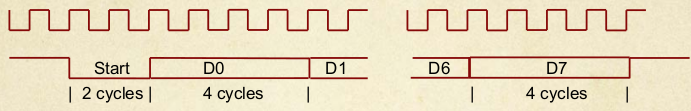
\includegraphics[width=.8\textwidth]{src/chrono_emetteur.jpg}
                        \captionof{figure}{Chronogramme émetteur}
                     \label{fig:trame}
                \end{figure}
        \end{itemize}
    \item    Chargement des bits tous les 4 cycles d'horloge après le front descendant du \textbf{start bit}
    \item    Quand la tranmission est finie, la trame est chargée dans le registre de sortie
    
\end{itemize}   
%fin de l'encadré
\end{tcolorbox}

\section{Architecture}\

\begin{tcolorbox}[colframe=Monokaimagenta,colback=white]
\paragraph{Architecture - Max 1/2 page}
Dessinez le schéma bloc complet de votre circuit. Ce circuit contient entre autre : shift-register, compteurs et machine d’état, avec les bus de données et les signaux de contrôle. Vous pouvez faire ce schéma bloc à la main (très proprement), ou en utilisant Logisim (mais avec le nom des signaux), ou avec un outil de dessin de votre choix.

Remplacez le texte ci-dessus par vos réponses (à l’intérieur du cadre rouge)\\

\begin{figure}[H]
    \centering
    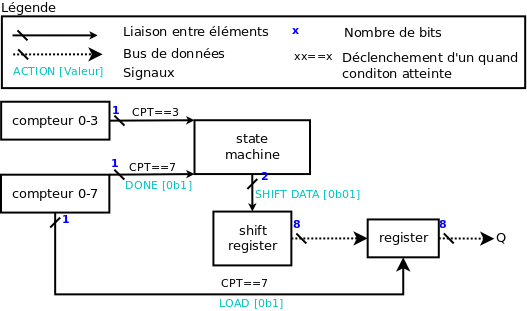
\includegraphics[width=.8\textwidth]{src/schema_bloc.png}
    \captionof{figure}{Schéma bloc}
    \label{fig:schem_bloc}
\end{figure}

Quand le compteur 0-3 atteint sa valeur maximum, il va envoyer un signal à la state machine qui elle va activer le shift register avec le signal 0b01 (décalage à droite).\\
Quand le compteur 0-7 aura atteint sa valeur maximum, il va envoyer un signal 0b1 à la state machine qui sera donc avertie que la transmission est finie et le registre peut charger les données.

\end{tcolorbox}

\section {Réalisation}
\subsection{Le bloc shift-register}
Ce bloc sur 8 bits a 4 modes de fonctionnement. Vous devez le refaire entièrement avec des bascules et des multiplexeurs.

\begin{tcolorbox}[colframe=Monokaimagenta,colback=white]
\paragraph{Conception et tests - Max 1 page}
\begin{figure}[H]
    \centering
    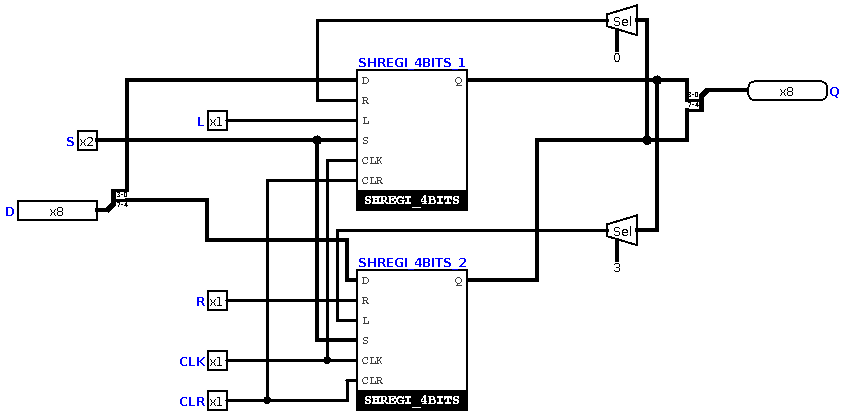
\includegraphics[width=.8\textwidth]{src/SHREGI_8BITS.png}
    \captionof{figure}{Bloc SHIFT REGISTER}
    \label{fig:SHREGI_8}
\end{figure}

Le shift register 8 bits est composé de 2 shift register 4 bits.  Ils ont comme entrée en commun l'horloge \textbf{CK}, \textbf{CLR} pour la remise à zéro et \textbf{S} qui comprend 4 états: 

\begin{center}
    \begin{tabular}{|c|c|c|c|}
        \hline
        S  & Action      & $Q+$ & Explications\\
        \hline
        00 & Hold        & $Q^+ = Q$   & Reste dans l'état passé \\
        01 & Load        & $Q^+ = D$   & Charge l'entier de l'entrée \\
        10 & Shift left  & $Q^+ = <<Q$ & Décale les bits à gauche \\
        11 & Shift right & $Q^+ = >>Q$ & Décale les bits à droite \\
        \hline    
    \end{tabular}    
\end{center}

Les entrées \textbf{R} et \textbf{L} sont utilisées lors d'un décalage, s'il se fait à droite les chiffres décalés vont être remplacés par des $0$ si \textbf{R} est actif et par des $1$ si \textbf{L} est actif, lors d'un décalage à gauche le schéma est inversé. Dans le cas d'une activation de ces 2 éléments, les chiffres seront remplacés par des $1$\\

Le byte est séparé en deux nibbles qui sont chacun en entrée \textbf{D} des register 4 bits.
Lorsqu'un décalage est fait, le dernier bit d'un registre doit être récupéré par le suivant, afin de ne pas perdre les bits décalés. Ainsi, pour le décalage à gauche, le bit [0] du shift register prenant en entrée D les bits [7:4] de l'octet (le deuxième SHREGI\footnote{Shift register} de l'illustration), doit être passé en entrée \textbf{R} du premier SHREGI. Ainsi, au moment du décalage à gauche, le bit[0] du deuxième SHREGI va bien être passé au premier SHREGI et il y aura une continuité dans le décalage.
Le même principe est appliqué pour le décalage à droite, mais cette fois c'est le bit [3] du 1\up{er} SHREGI qui va être donné en entrée \textbf{L} du 2\up{ème} SHREGI.

\paragraph{Les tests ont été effectués avec un chronogramme (voir \ref{fig:chrono_shregi8}) }. Dans un premier le chronogramme incrémente sa valeur, ensuite l'entrée \textbf{S} passe à $01$, ce qui permet de charger les données dans \textbf{D}, ensuite \textbf{S} se met en mode $10$ et les bits se retrouvent décalés vers la droite. Dans un 2\up{ème} temps, \textbf{D} est composé de $0$ donc \textbf{S} charge à nouveau les données et s'active cette fois avec $11$ pour un décalage à droite.
  
\end{tcolorbox}

\subsection{Le bloc compteur 0-3}
Le premier compteur demandé compte de 0 à 3. Ce compteur comprend une entrée de remise à 0 synchrone et une sortie indiquant que le compteur a atteint sa valeur maximum.
\begin{tcolorbox}[colframe=Monokaimagenta,colback=white]
\paragraph{Conception et tests - Max 1 page }
\begin{figure}[H]
\centering
    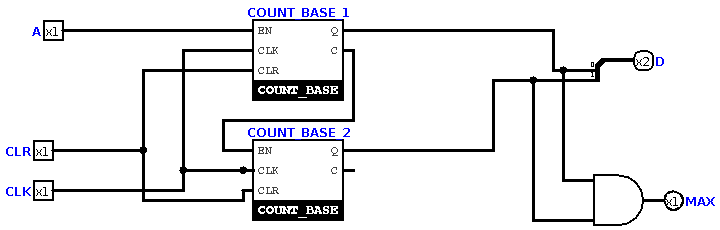
\includegraphics[width=.8\textwidth]{src/COUNT_4BITS.png}
    \captionof{figure}{Compteur 0\-3}
    \label{fig:count4bits}
\end{figure}
Insérez une capture d’écran pour présenter votre bloc compteur 0-3. Expliquez sa réalisation et son fonctionnement.
Indiquez comment vous avez testé les différents modes de fonctionnement afin de le valider. Vous pouvez ajouter un chronogramme.
Remplacez le texte ci-dessus par vos réponses (à l’intérieur du cadre rouge)


Ce bloc est composé d'un bloc de base (voir \ref{fig:countBase}) qui s'occupe uniqument de changer l'étât une bascule D, ce qui aura comme effet de "compter" lorsque qu'il est connecté avec d'autres de ces blocs.\\
Dans notre cas, ce circuit va incérmenter sa valeur jusqu'à arriver à $3$, lorsque qu'il a atteint ce nombre, la sortie \textbf{MAXb} s'activera pour indiquer que le compteur est arrivé à la fin.

\paragraph{Définition des entrées}
\begin{itemize}

    \item     \textbf{A} Active le compteur
    \item     \textbf{CLK} Permet de connecter l'horloge du circuit "maître"
    \item     \textbf{CLR} Remise à zéro du compteur
\end{itemize}

\paragraph{Définition des sorties}
\begin{itemize}

    \item     \textbf{MAX} S'active lorsque que le compteur à atteint sa valeur maximum, c'est-à-dire 3.
    \item     \textbf{D} Affiche l'état du compteur
\end{itemize}



\paragraph{Les tests ont été effectués avec le chronogramme ci-dessous}. Lorsque que le compteur atteint la valeur $3$ la sortie \textbf{MAX} est active et le la sortie \textbf{D} incrémente bel et bien sa valeur.

\begin{figure}[H]
\centering
    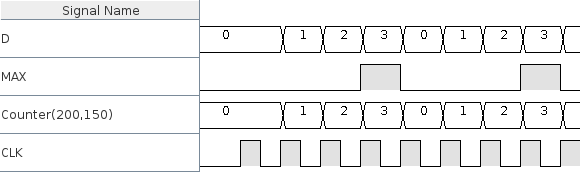
\includegraphics[width=.8\textwidth]{src/chrono_COUNT_4.png}
    \captionof{figure}{Compteur 0-3}
    \label{fig:count4bits}
\end{figure}

\end{tcolorbox}
\subsection{Le bloc compteur 0-7}
Le deuxième compteur demandé compte de 0 à 7. Ce compteur comprend une entrée de remise à 0 synchrone, une entrée enable pour l’activer et une sortie indiquant que le compteur a atteint sa valeur maximum.
\begin{tcolorbox}[colframe=Monokaimagenta,colback=white]
\paragraph{Conception et tests - Max 1 page}
Insérez une capture d’écran pour présenter votre bloc compteur 0-7. Expliquez sa réalisation et son fonctionnement. Inutile de reprendre les explications du paragraphe précédent 3.2. Expliquez simplement ce que vous avez dû changer ou rajouter pour passer du compteur 0-3 au compteur 0-7.
Indiquez comment vous avez testé les différents modes de fonctionnement afin de le valider. Vous pouvez ajouter un chronogramme.
Remplacez le texte ci-dessus par vos réponses (à l’intérieur du cadre rouge)

\begin{figure}[H]
\centering
    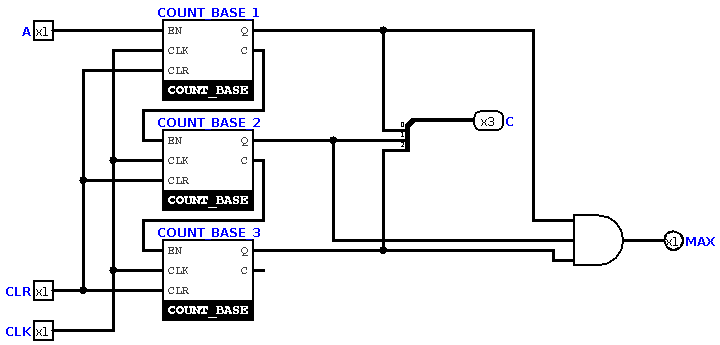
\includegraphics[width=.8\textwidth]{src/COUNT_8BITS.png}
    \captionof{figure}{Compteur 0\-3}
    \label{fig:count4bits}
\end{figure}

Vu que nous avons un circuit de base qui permettrait de créer n compteurs, l'ajout d'un bloc de ce circuit à été nécessaire et la sortie \textbf{D} et \textbf{MAX} ont aussi été adaptés.

\paragraph{Les tests ont été effectués avec le chronogramme ci-dessous}. Lorsque que le compteur atteint la valeur $7$ la sortie \textbf{MAX} est active et le la sortie \textbf{D} incrémente bel et bien sa valeur.
\begin{figure}[H]
\centering
    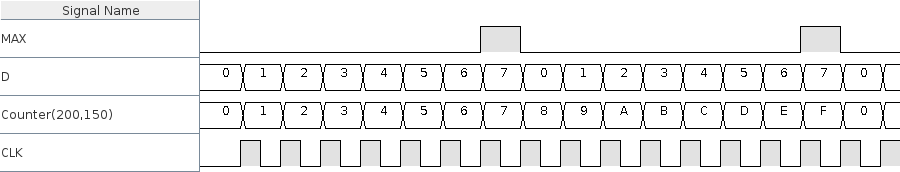
\includegraphics[width=.8\textwidth]{src/chrono_COUNT_8.png}
    \captionof{figure}{Compteur 0-7}
    \label{fig:count8bits}
\end{figure}



\end{tcolorbox}
\subsection{La machine d’état}
Cette machine d’état de type 1 parmi M contrôle les deux compteurs et le shift register. 
\begin{tcolorbox}[colframe=Monokaimagenta,colback=white]
\paragraph{Conception Max 3 pages}
Insérez un graphe des états et une table des états. Donnez des explications sur le fonctionnement de votre machine. Quel est son Type ?
Donnez les équations des états futurs et insérez une capture d’écran de la réalisation de votre machine.
Remplacez le texte ci-dessus par vos réponses (à l’intérieur du cadre rouge)\\

\begin{figure}[H]
\centering
    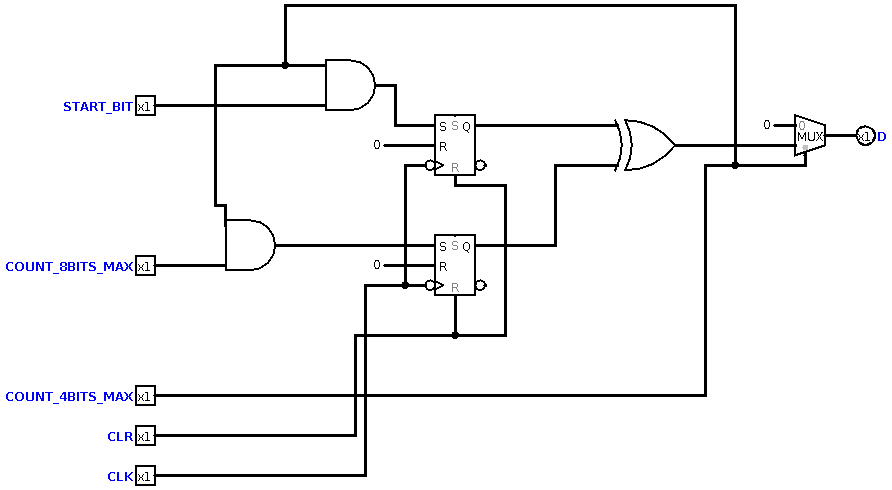
\includegraphics[width=.8\textwidth]{src/STAMAC.png}
    \captionof{figure}{State machine}
    \label{fig:stamac}
\end{figure}


Cette machine d'état prend en entrée le compteur 4 bits, le compteur 8 bits et le bit envoyé par l'émetteur. Les bascules bistables sont de type S-R car il fallait qu'elle ne change pas d'état après être passée à $1$ au flanc montant. Cette machine d'état va renvoyer un $1$ si un $0$ à été transmis comme signal de départ et si 8 coups d'horloges n'ont pas encore été atteints.\\
La première bascule prend en entrée l'inverse du bit envoyé par l'émetteur (de façon à ce que l'horloge passe à $1$ lorsque le bit envoyé est un $0$). Ainsi, à chaque coup d'horloge, celle de la première bascule va passer à 1, et si l'entrée \textbf{S} de la bascule est à $1$ (et donc le bit envoyé par l'émetteur à $0$), l'état de la bascule va passer à 1 et y rester. Ainsi, on sait que le bit qui signale le départ à été envoyé.\\
La deuxième bascule prend en entrée le compteur 8 bits. Ainsi, à chaque coup d'horloge, la bascule va "contrôler" que l'on ait pas atteint la fin du mot. Si l'entrée est à $1$ lorsque le compteur 8 bit annonce la fin du mot, la bascule change d'état et y reste.\\
Au bout du circuit, une porte XOR permet de savoir si les deux bascules ne sont pas au même état.
Ainsi, au départ, la sortie est à 0. Dès qu'un zéro est transmis par l'émetteur, la première bascule passe à $1$, et la sortie sera à $1$ également. Puis, dès qu'on atteint les 8 coups d'horloge, la deuxième bascule passe à $1$ aussi, et la sortie passe donc définitivement à $0$.\\
Enfin, un MUX tout à la fin enverra en sortie la constante $0$ tant que le COUNT\_4BIT\_MAX est à $0$, et enverra en sortie le résultat du XOR si COUNT\_4BITS est à $1$. Ainsi, on prend en compte l'état de la machine d'état chaque 4 coups d'horloge (puisque les bits émis par l'émetteurs son récupérés chaque 4 coups d'horloge).\\
Cette machine d'état est de type 1 parmi N.

Équations de la machine d'état:
\textbf{Q0+} = NOT(LAST\_BIT)
\textbf{Q1+} = COUNT\_8BITS\_MAX
\textbf{D} = ( (NOT(LAST\_BIT)  XOR COUNT\_8BITS\_MAX ) COUNT\_4BITS\_MAX

Table des états:
\begin{center}
    \begin{tabular}{| c c c || c c |}
    \hline
    COUNT8B & LASTB & COUNT4B & D & ETAT
    0 & 0 & 0 & 0 & Hold \\ \hline
    0 & 0 & 1 & 1 & Load \\ \hline
    0 & 1 & 0 & 0 & Hold \\ \hline
    0 & 1 & 1 & 0 & Hold \\ \hline
    1 & 0 & 0 & 0 & Hold \\ \hline
    1 & 0 & 1 & 0 & Hold \\ \hline
    1 & 1 & 0 & 0 & Hold \\ \hline
    1 & 1 & 1 & 1 & Stop \\ \hline
    \end{tabular}
\end{center}
\end{tcolorbox}

\begin{figure}[H]
\centering
    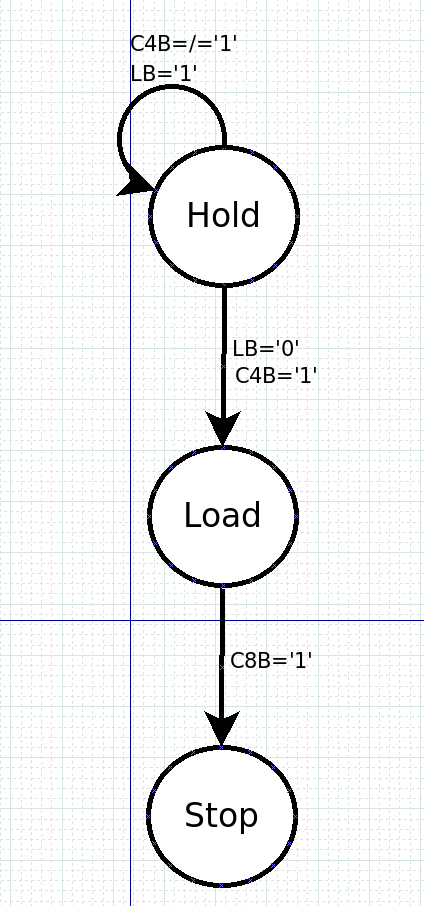
\includegraphics[width=.8\textwidth]{src/stamac2.png}
    \captionof{figure}{States}
    \label{fig:stamac2}
\end{figure}

\section {Intégration et simulation}
\subsection{Intégration}
Suivant votre partie à concevoir, vous devez réaliser l’UART en interconnectant les différents blocs. 
\begin{tcolorbox}[colframe=Monokaimagenta,colback=white]
\paragraph{Réalisation et simulation Logisim - Max 1 page}
Insérez une capture d’écran de l’UART complet sous Logisim
Expliquez le fonctionnement global de l’UART\\

\begin{figure}[H]
\centering
    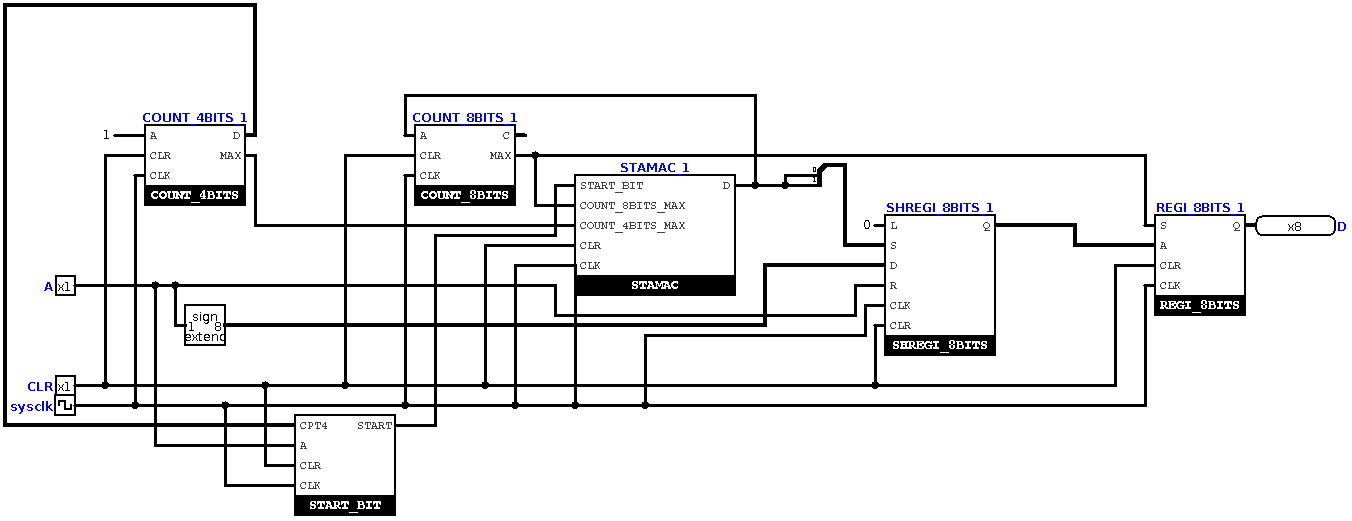
\includegraphics[width=1\textwidth]{src/UART.png}
    \captionof{figure}{Circuit de base des compteurs}
    \label{fig:countBase}
\end{figure}

L'UART est composé d'un compteur 4 bits(voir \ref{fig:count4bits}), d'un compteur 8 bits(voir \ref{fig:count8bits}), d'une machine d'état (voir \ref{fig:stamac}), d'un shift reister 8 bits (voir \ref{fig:SHREGI_8}) ainsi qu'un register de sortie 8 bits (voir \ref{fig:SHREGI_8}).\\    
Les différentes entrées de l'UART sont:
\begin{itemize}
    \item     \textbf{A} Bit envoyé par l'émetteur
    \item     \textbf{CLR} Remise à zéro du compteur
    \item     \textbf{sysclk} Horloge principale, reliée à tous les circuits
\end{itemize}
En sortie:
\begin{itemize}
    \item     \textbf{D} Affiche la sortie du registre, donc la séquence de 8 bits transmise, après $8*4$ coups d'horloge.
\end{itemize}
Le fonctionnement global de la machine d'état est le suivant:
Le bit A va être transmis à un shift register, qui sera activé seulement lorsque la machine d'état lui transmettra un $1$. Cette machine d'état passer à l'état "activé" lorsque elle reçoit un 0. Les bits sont reçus chaque 4 coups d'horloge, et on doit compter 8 bits à partir du début de la transmission, d'où les compteurs 4 et 8 bits. Enfin, un registre load les 8 bits reçus.\\
Le shift register n'est pas activé d'emblée. Son entrée \textbf{S} reçoit la sortie de la machine d'état, dont l'état passera à l'état "activé" au moment où l'on veut commencer à recevoir les bits, c'est-à-dire quand un $0$ est transmis.
Lorsqu'un premier $0$ est transmis par l'émetteur, la machine d'état va changer d'état et activer ou non le shift register en lui passant le bit de sortie dans son entrée \textbf{S} (le même bit est donné à \textbf{S0} et \texbf{S1}). La sortie de la machine d'état va être prise en compte chaque 4 coups d'horloge, le reste du temps elle reste à 0. Ainsi, le shift register va être activé uniquement chaque 4 coups d'horloge (comme requis), et ce 8 fois (le temps de recevoir le mot en entier).\\
Le compteur 4 bits prend un $1$ en entrée \textbf{A} car il doit compter continuellement, puisqu'il faut recevoir un bit de l'émetteur chaque 4 coups d'horloge. Le compteur 8 bits, lui, doit commencer à compter seulemement lorsqu'on doit recevoir les bits de l'émetteur, et doit considerer 4 coups d'horloge comme un seul. Il prend donc en entrée la sortie de la machine d'état, qui aura un $1$ en sortie à chaque 4 coups d'horloge dès l'instant où un 0 est transmis par l'émetteur, donc il va bien compter un bit chaque 4 coups d'horloge. Ainsi, le compteur 8 bits arrivera à 8 lorsqu'il y aura eu 32 coups d'horloge.\\
Le register de sortie a pour rôle de charger les 8 bits dans une sortie lorsqu'ils ont été transmis. Il prend donc en entrée A la sortie du shift register, qui contiendra les bits reçus. En entrée \textbf{S}, il prend la sortie du compteur 8 bits, ainsi c'est seulement à la fin de la réception des 8 bits que les bits vont être chargé. Le reste du temps, les bits seront conservés (le register est sur "hold").
Ainsi, on a bien une réception de 8 bits loadés dans une sortie après $8*4$ coups d'horloge après le signal donné par un bit à $0$ transmis au début.

\end{tcolorbox}
 \subsection{Simulation sous Logisim}
L’UART réalisé est ensuite testé en simulation sous Logisim.
\begin{tcolorbox}[colframe=Monokaimagenta,colback=white]
\paragraph{Réalisation et simulation Logisim - Max 2 pages}
Indiquez comment vous simulez votre UART sous Logisim (seul ou avec le générateur fourni), ET avec un UART d’un autre groupe (indiquez quel groupe)
Insérez un ou plusieurs chronogrammes, annotez-le(s) et expliquez pourquoi le fonctionnement est correct et conforme aux spécifications.
Remplacez le texte ci-dessus par vos réponses (à l’intérieur du cadre rouge)
Pour simuler l'UART sous logisim, nous avons mis la fréquence de l'horloge sur 2Hz, et nous avons mis l'entrée \textbf{A} à $1$, pour que la transmission ne démarre pas immédiatement. Nous avons aussi ajouté une sortie au shift register, car cela nous permettait de suivre l'avancement des bits au moment de la tranmission.\\
Nous avons lancé l'horloge, et après un nombre arbitraire de coups d'horloge, nous avons passé l'entrée \textbf{A} de $1$ à $0$. Nous avons pu constater le début de la tranmission des bits, en variant l'entrée \textbf{A}, et nous avons compté les coups d'horloge pour nous assurer que les compteurs fonctionnaient correctement.
Nous avons aussi testé chaque circuit indépendamment.
\\
\end{tcolorbox}
 \subsection{Synthèse et test de fonctionnement réel}
Synthèse et configuration du matériel, test de fonctionnement.
L’UART finalement synthétisé et chargé dans une carte, une carte émetteur sera reliée à une carte récepteur afin de tester une transmission de données. 


\begin{tcolorbox}[colframe=Monokaimagenta,colback=white]

Indiquez comment vous faites le test (et avec un groupe différent de la simulation). Quelles données choisissez-vous pour faire les essais ?Vous devez faire valider votre circuit en fonctionnement au quiprofesseur ou à l’assistant
Commentez brièvement votre expérience dans cette étape en mentionnant, par exemple, des éventuelles difficultés à faire fonctionner le circuit ou à configurer la carte, etc.
Remplacez le texte ci-dessus par vos réponses (à l’intérieur du cadre rouge)\\

\paragraph{Essais avec une carte - Max 1 page}
Pour l'essai avec la carte, nous avons pris une fréquence à 32Hz, et nous avons téléchargé l'UART sur la carte avec les données suivantes:
\begin{itemize}
    \item     \textbf{A} les 8 bits transmis par l'émetteur
    \item     \textbf{CLR} la remise à zéro du compteur
    \item     \textbf{CLK} l'horloge
\end{itemize}

La carte est branchée à l'ordinateur, ainsi qu'à une console. Le test se faisait avec un autre groupe, qui avait du faire un émetteur. L'objectif était donc que ce groupe émette une série de bits que nous puissions recevoir.
Les 8 bits de la donnée reçue ont été connectés aux 8 LED de la console, pour pouvoir contrôler la bonne récpection des bits tranmis par l'émetteur. L'entrée "reset" a été connectée au bouton \textbs{SW8}. L'entrée A, qui reçoit 1 à 1 les bits transmis, a été connectée au pin \textbs{MEZ1}. Le fil reliant les deux cartes (celle du groupe émetteur et la notre) se trouvait sur ce connecteur \textbs{MEZ1}.\\
Nous avons dû télécharger notre UART sur la carte, et brancher les deux cartes ensemble.
Nous avons rencontré passablement de difficultés lors de cette étape. Tout d'abord, nous ne pouvions pas charger notre UART sur la carte, car, à la base, les horloges étaient reliées au compteur 4 bits, de sorte à compter un coup d'horloge chaque 4 coups. Malheureusement, nous avons constaté que, de cette manière, les bascules n'étaient pas synchronisées. Nous avons donc dû modifier nos circuits en conséquence.\\
Un autre poblème que nous avons rencontré, est qu'il n'y avait pas de moyen de mise à zéro sur tous nos circuits, donc lorsque l'on choisissait de remettre la carte à zéro, tout n'était pas remis à son état initial.\\
Nous avons aussi fait l'erreur d'essayer de mettre une horloge dans chaque circuit contenu dans l'UART, mais nous avons rapidement corrigé cela pour remettre une horloge principale et de simples pin dans les circuits.\\
Après cela, nous avons retesté notre circuit sur carte, avec comme l'émetteur de M.Matthey. Au final, le résultat sur la carte n'était tout de même pas concluant, car trois $0$ s'affichent à la fin, indépendamment de la série de bits envoyés. Nous n'avons pas trouvé la source de ce problème, même s'il vient probablement d'un compteur. Cependant, les autres bits transmis sont corrects. Sur logisim, l'UART fonctionne correctement.

\end{tcolorbox}
\section {Conclusion}
\begin{tcolorbox}[colframe=Monokaimagenta,colback=white]
\paragraph{Conclusion - Max 1/2 page}
Ce laboratoire était assez complet et regroupait globalement ce que nous avions vu jusqu'à maintenant. Il nous a demandé d'investir un temps assez conséquent, notamment parce que nous avions fait plusieurs erreurs dans les circuits, que nous avons parfois mis du temps à trouver.\\
La plus grosse difficulté a été le test sur carte. Lorsque que nous l'avons fait la permière fois en classe, des erreurs dans les circuits nous ont empêché de le réaliser correctement, et nous avons dû effectuer de nombreuses modifications afin de pouvoir passer l'UART sur la carte. Par la suite, nous avons pu le mettre sur carte pour tester, mais le résultat était peu concluant. Comme cela semblait fonctionner sur logisim, ce résultat était assez frustrant.\\
Nous avons aussi pris un certain temps pour réaliser l'UART, à laquelle il manquait, au début, le bloc register, et lier tous les circuits déjà faits entre eux. De plus, nous pensions pouvoir mettre en entrée des horloges les compteurs 4 et 8 bits, ce qui n'était, en réalité, pas faisable. Nous avons donc dû trouver un moyen de rendre les horloges dépendantes des compteurs sans toutefois les y connecter, ce qui a été une difficulé aussi.\\
En conclusion, la façon dont sont faits nos circuits n'est pas vraiment optimale, et le test sur carte est peu concluant, mais l'ensemble fonctionne et nous avons pu apprendre des erreurs que nous avons commises, et mieux comprendre le fonctionnement des machines d'état. Ce laboratoire était donc enrichissant.

\end{tcolorbox}

\section{Lexique}
\begin{itemize}
    \item     SHREGI: Shift Register
    \item     REGI: Register
    \item     STAMAC: State Machine
\end{itemize}


\section{Annexe}


\begin{figure}[H]
\centering
    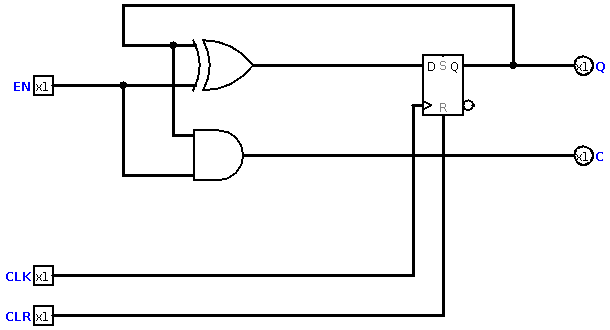
\includegraphics[width=.8\textwidth]{src/COUNT_BASE.png}
    \captionof{figure}{Circuit de base des compteurs}
    \label{fig:countBase}
\end{figure}

\begin{figure}[H]
\centering
    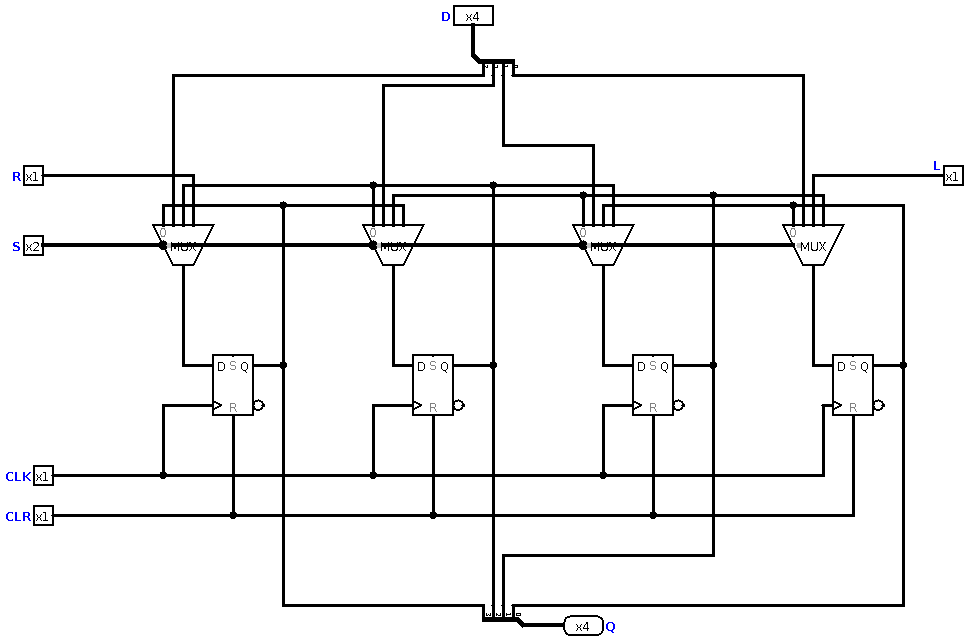
\includegraphics[width=.8\textwidth]{src/SHREGI_4BITS.png}
    \captionof{figure}{SHIFT REGISTER 4BITS}
    \label{fig:shregi4}
\end{figure}

\begin{figure}[H]
\centering
    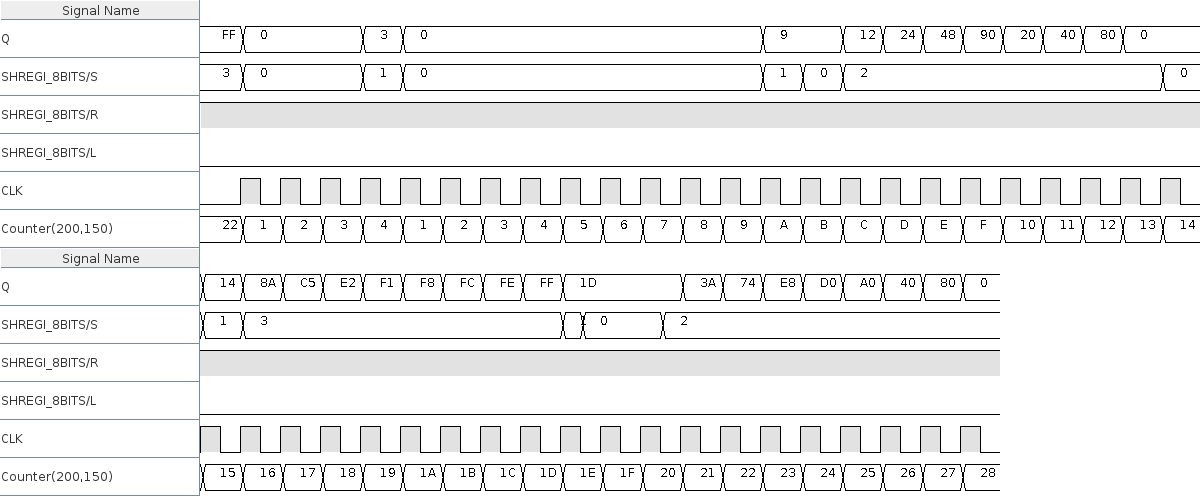
\includegraphics[width=1\textwidth]{src/chrono_SHREG_8BITS.png}
    \captionof{figure}{Chronogramme Shift Register 8bits}
    \label{fig:chrono_shregi8}
    Note: les premières données FF et 3 ne doivent pas être prises en compte
\end{figure}


\end{document}